\chapter{Classification of animate and inanimate objects}
\label{chap:bmt-exp} % id kapitoly pre prikaz ref

In this chapter, we focused on existing model Binary mean teacher, that is derived from semi-supervised model Mean Teacher, and is used for binary classification. Our task was to classify images of animate and inanimate objects. We introduced our custom made dataset, that contains images from standard dataset CIFAR10 which we relabeled into only two classes. The main goal of this experiment was to test performance of the Binary mean teacher model. We have done several experiments with this new dataset and compared semi-supervised model performance with supervised baseline.


\section{Task description}

Our goal was to find out, whether model is able to discover features that are specific for appearence of living creatures and others that define lifeless objects and differenciate these two classes of objects.
Simply, our task was classification of images into two classes - animate objects and inanimate objects. 

\section{Dataset}
\label{dataset-cifar10}

We chose to transform and use standard CIFAR10 dataset \cite{krizhevsky2009} which consists of $60000$ colour images with resolution $32 \times 32$ pixels in 10 classes (bird, cat, deer, dog, frog, horse, airplane, automobile, ship, truck), with $6000$ images per class. 

In this experiment, we transformed dataset from original ten classes into two - animate and inanimate. Animate class
was formed of images from original classes bird, cat, deer, dog, frog and horse. Inanimate class consisted of images that was in originally in classes airplane, automobile, ship and truck. Samples from dataset are shown in figure \ref{fig:cifar10}.

\begin{figure}
    \centering
    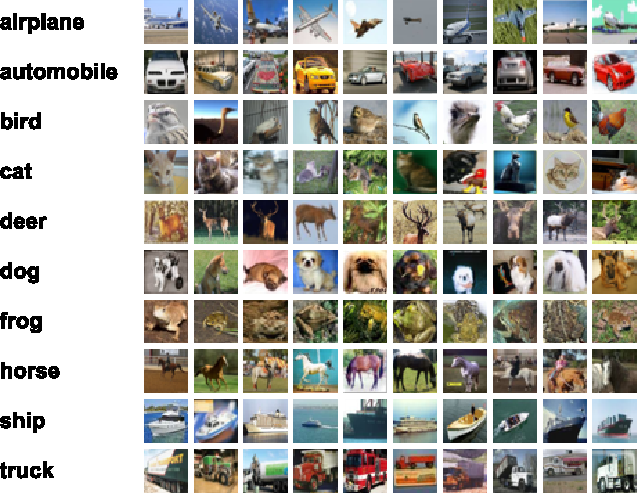
\includegraphics{figs/cifar10-sample-fig.pdf}
    \caption{Samples from CIFAR10 dataset}
    \label{fig:cifar10}
\end{figure}


\section{Models}

We wanted to compare semi-supervised model performance with supervised model, to find out how unsupervised part of model support learning. As far as the task was designed for binary classification, we decided to use semi-supervised model Binary mean teacher described in section \ref{bmt}. As a baseline we used supervied feedforward neural network with the same layer architecture as semi-supervised model. Our dataset was completely new, so we needed to compute accuracy for both models with various of different hyperparameters. 
 
\subsection{Network description}
Architecture of hidden layers was taken from Muhammad Sarmad's github repository \footnote{\url{https://github.com/iSarmad/MeanTeacher-SNTG-HybridNet}}, from his implementation of Mean Teacher model. Neural net had $25$ layers described in table \ref{layers} with ReLU as activation functions for all layers except last two. In last two layers, he used sigmoid activation function.


\begin{table}[ht]
    \centering
    \begin{tabular}{ |c|} 
     \hline
            hidden layer with parameters \\
            \hline
            3 $\times$ BatchNorm2d(128) \\
            Conv2d(3, 128, 3,padding=1) \\
            2 $\times$ Conv2d(128, 128, 3,padding=1) \\
            MaxPool2d(2, 2)\\
            Dropout(0.5)\\
            3 $\times$ BatchNorm2d(256)\\
            Conv2d(128, 256, 3, padding=1)\\
            2 $\times$ Conv2d(256, 256, 3, padding=1)\\
            MaxPool2d(2, 2)\\
            Dropout(0.5)\\
            BatchNorm2d(512)\\
            BatchNorm2d(256)\\
            BatchNorm2d(128)\\
            Conv2d(256, 512, 3)\\
            Conv2d(512, 256, 1)\\
            Conv2d(256, 128, 1)\\
            AvgPool2d(6,6)\\
            nn.Linear(128, 1)\\
            BatchNorm1d(1)\\
     \hline
    \end{tabular}
    \caption{Table of layers in network}
    \label{layers}
\end{table}

\subsection{Implementation}
We developed this experiment in this GitHub repository \footnote{\url{https://github.com/Sabka/DT-MT}}. Repository contains code for dataset transformation and the experiments.
Core of the model implementation was taken from Sarmad's Mean Teaches. We used his hidden architecture, but changed the last layer dimension to one, which is necessary for binary classification. We also changed the unsupervised loss calculation to use representation from last convolution layer instead of network output. These changes were necessary to transform Mean Teacher into Binary mean teacher model.
During developement, we validated, that it is necessary to use feature vectors from last convolutional layer when computing MSE. It was esential for network convergence. 

\subsection{Baseline}
Our baseline was deep network trained on same portion of labeled data. We will run fully supervised network and compouted accuracy on our custom made dataset. As we mentioned, this network had the same architecture as student or teacher network, so difference in accuracy should show the effect of using additional information from unsupervised loss in learning of semi-supervised model. 

We trained network on $4000$ labeled data. Training consisted of 30 epochs, learning rate was set to $0.5$, optimizer was SGD. Best accuracy net achieved was \textbf{93\%}, as evaluation on 10000 labeled samples.


\section{Training}
\label{bmt:training}
We trained all networks for 30 epochs and used SGD optimizer. Ratio of labeled and unlabeled samples in training set was constant and was $4000:46000$. Network was evaluated on $10000$ labeled samples. As image augmentations, we used  flipping and rotation.

\section{Experiments}

We tried 3 different subtasks. First one focused on looking for learning rate that gives good results for semi-supervised model, second discovered how different type of augmentation influence model accuracy and last one was about trying different amount of labeled data in training set and looking whether unlabeled data which semi-superised model use helped its performance in comparison to supervised model with only labeled data.


\subsection{Learning rate}
We tried several values of learning rate hyperparameter and trained only semi-supervised model with other parameters set as described in section \ref{bmt:training}. Our goal was to observe, which values of learning rate were good for the task. We state table \ref{bmt:lr} which contains best learning rate with accuracies.

\begin{table}[h]
    \centering
    \begin{tabular}{ |c|c|} 
     \hline

     Learning rate & Student validation acc\\
     \hline
     0.05 & 87\% \\
     0.1 &  89\% \\
     0.5 & 91\% \\
     \hline
    \end{tabular}
    \caption{Learning rate accuracies}
    \label{bmt:lr}
\end{table}

\subsection{Different augmentation}
In next experiment, we tried to use color augmentation for input data. We chose Pytorch ColorJitter, which change colors according to parameters brightness, contrast, saturation and hue. The result of transformation can look like in image \ref{jitter}.
Our best model with data augmented by ColorJitter, on $4000$ labeled datapoints and $46000$ unlabed datapoints and learning rate $0.5$ achieved accuracy \textbf{91\%}, which is not better than with same hyperparameters and only flip and rotate augmentation.
\color{red}  TODO ozdrojovat ColorJitter + zacitovat ako im to pomohlo pri batohoch
\color{black}
\begin{figure}[!h]
    \centering
    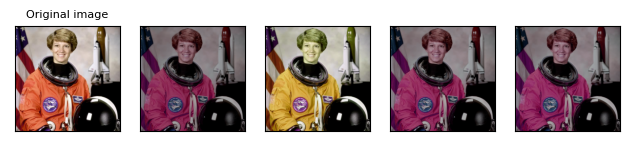
\includegraphics[width=1\textwidth]{figs/jitter.png}
    \caption{Color Jitter augmentation example \cite{colorjitter}}
    \label{jitter}
\end{figure}


\subsection{Size of portion of labeled data}

In this final experiment, we tended was to show, how unlabeled examples helped model to learn better when there were  smaller portion of labeled examples, which is the main goal of semi-supervised learning. We introduced new hyperparameter - portion of labeled data and monitor accuracy of net and computed new baselines. For each portions of labeled data, we trained supervised model. The results are shown in table \ref{portions}. Highlighted results show cases where Binary Mean Teacher model achived better accuracy than baseline model.

\begin{table}[h]
    \centering
    \begin{tabular}{ |c|c|c|c|} 
     \hline

     portion & LR & Student validation acc & Baseline (with same portion)\\
     \hline
     
     100 & 0.1 & \color{purple}  78\%   &  60\% \\ 
     100 & 0.5 & \color{purple} 80\%  & 60\% \\
     500 & 0.5 & \color{purple} 88\% &  85\% \\
     500 & 0.1 & \color{purple} 88\% &  85\% \\
     1000 & 0.1 & \color{purple}89\% &  83\% \\
     1000 & 0.5 & \color{purple}90\% &  83\%  \\
     4000 & 0.1 & 89\% & 93\% \\
     4000 & 0.5 & 91\% & 93\%  \\
     
     \hline
    \end{tabular}
    \caption{Comparison of models}
    \label{portions}
\end{table}


\section{Discussion of results} 
First experiment showed, that $4000$ labeled samples are enough for supervised model to train well. Semi-supervised model didn't achieved this high accuracy  even when trying different values of learning rate hyperparameter.

In second experiment, we tried to use different augmentation - change of colors in the image. In this case, model did not work any better than using only flip and rotation. Accuracy stayed the same.


Last experiment focussed on how different size of portion of labeled data influenced model's results. This showed that semi-supervised model worked much better for smaller portions of data, when supervised model wasn't able to acomplish that high accuracy. This experiment showed, that huge amount of unlabeled data used for trainig of semi-supervised model helped its performance.

There are several things about Binary Mean Teacher model, that could be studied in future. We recommend future research to focus on more complex architectures, which was not able for us, because of our hardware limitations. Study of different hyperparameters, such as EMA decay or consistency cost weight in weighted sum of costs could also help to reach better performance.


